\documentclass{article}\usepackage[]{graphicx}\usepackage[]{color}
% maxwidth is the original width if it is less than linewidth
% otherwise use linewidth (to make sure the graphics do not exceed the margin)
\makeatletter
\def\maxwidth{ %
  \ifdim\Gin@nat@width>\linewidth
    \linewidth
  \else
    \Gin@nat@width
  \fi
}
\makeatother

\definecolor{fgcolor}{rgb}{0.345, 0.345, 0.345}
\newcommand{\hlnum}[1]{\textcolor[rgb]{0.686,0.059,0.569}{#1}}%
\newcommand{\hlstr}[1]{\textcolor[rgb]{0.192,0.494,0.8}{#1}}%
\newcommand{\hlcom}[1]{\textcolor[rgb]{0.678,0.584,0.686}{\textit{#1}}}%
\newcommand{\hlopt}[1]{\textcolor[rgb]{0,0,0}{#1}}%
\newcommand{\hlstd}[1]{\textcolor[rgb]{0.345,0.345,0.345}{#1}}%
\newcommand{\hlkwa}[1]{\textcolor[rgb]{0.161,0.373,0.58}{\textbf{#1}}}%
\newcommand{\hlkwb}[1]{\textcolor[rgb]{0.69,0.353,0.396}{#1}}%
\newcommand{\hlkwc}[1]{\textcolor[rgb]{0.333,0.667,0.333}{#1}}%
\newcommand{\hlkwd}[1]{\textcolor[rgb]{0.737,0.353,0.396}{\textbf{#1}}}%
\let\hlipl\hlkwb

\usepackage{framed}
\makeatletter
\newenvironment{kframe}{%
 \def\at@end@of@kframe{}%
 \ifinner\ifhmode%
  \def\at@end@of@kframe{\end{minipage}}%
  \begin{minipage}{\columnwidth}%
 \fi\fi%
 \def\FrameCommand##1{\hskip\@totalleftmargin \hskip-\fboxsep
 \colorbox{shadecolor}{##1}\hskip-\fboxsep
     % There is no \\@totalrightmargin, so:
     \hskip-\linewidth \hskip-\@totalleftmargin \hskip\columnwidth}%
 \MakeFramed {\advance\hsize-\width
   \@totalleftmargin\z@ \linewidth\hsize
   \@setminipage}}%
 {\par\unskip\endMakeFramed%
 \at@end@of@kframe}
\makeatother

\definecolor{shadecolor}{rgb}{.97, .97, .97}
\definecolor{messagecolor}{rgb}{0, 0, 0}
\definecolor{warningcolor}{rgb}{1, 0, 1}
\definecolor{errorcolor}{rgb}{1, 0, 0}
\newenvironment{knitrout}{}{} % an empty environment to be redefined in TeX

\usepackage{alltt}
\usepackage[sc]{mathpazo}
\renewcommand{\sfdefault}{lmss}
\renewcommand{\ttdefault}{lmtt}
\usepackage[T1]{fontenc}
\usepackage{geometry}
\geometry{verbose,tmargin=2.5cm,bmargin=2.5cm,lmargin=2.5cm,rmargin=2.5cm}
\setcounter{secnumdepth}{2}
\setcounter{tocdepth}{2}
\usepackage[unicode=true,pdfusetitle,
 bookmarks=true,bookmarksnumbered=true,bookmarksopen=true,bookmarksopenlevel=2,
 breaklinks=false,pdfborder={0 0 1},backref=false,colorlinks=false]
 {hyperref}
\hypersetup{
 pdfstartview={XYZ null null 1}}

\makeatletter
%%%%%%%%%%%%%%%%%%%%%%%%%%%%%% User specified LaTeX commands.
\renewcommand{\textfraction}{0.05}
\renewcommand{\topfraction}{0.8}
\renewcommand{\bottomfraction}{0.8}
\renewcommand{\floatpagefraction}{0.75}

\makeatother
\IfFileExists{upquote.sty}{\usepackage{upquote}}{}
\begin{document}








The results below are generated from an R script.

\begin{knitrout}
\definecolor{shadecolor}{rgb}{0.969, 0.969, 0.969}\color{fgcolor}\begin{kframe}
\begin{alltt}
\hlcom{#3 - constructing the spatial weight matrix}
\hlkwd{library}\hlstd{(spdep)}
\end{alltt}


{\ttfamily\noindent\itshape\color{messagecolor}{\#\# Loading required package: sp}}

{\ttfamily\noindent\itshape\color{messagecolor}{\#\# Loading required package: spData}}

{\ttfamily\noindent\itshape\color{messagecolor}{\#\# To access larger datasets in this package, install the spDataLarge package with:\\\#\# `install.packages('spDataLarge', repos='https://nowosad.github.io/drat/',\\\#\# type='source')`}}

{\ttfamily\noindent\itshape\color{messagecolor}{\#\# Loading required package: sf}}

{\ttfamily\noindent\itshape\color{messagecolor}{\#\# Linking to GEOS 3.9.1, GDAL 3.2.3, PROJ 7.2.1}}\begin{alltt}
\hlstd{z1} \hlkwb{<-} \hlkwd{c}\hlstd{(}\hlnum{5}\hlstd{,}\hlnum{1}\hlstd{,}\hlnum{2}\hlstd{,}\hlnum{4}\hlstd{)}
\hlstd{z2} \hlkwb{<-} \hlkwd{c}\hlstd{(}\hlnum{3}\hlstd{,}\hlnum{4}\hlstd{,}\hlnum{2}\hlstd{,}\hlnum{1}\hlstd{)}
\hlstd{data} \hlkwb{<-} \hlkwd{cbind}\hlstd{(z1,z2)}
\hlstd{mdist} \hlkwb{<-} \hlkwd{sqrt}\hlstd{(}\hlkwd{sum}\hlstd{(}\hlkwd{diff}\hlstd{(}\hlkwd{apply}\hlstd{(data,} \hlnum{2}\hlstd{, range))}\hlopt{^}\hlnum{2}\hlstd{))}
\hlstd{dnb} \hlkwb{=} \hlkwd{dnearneigh}\hlstd{(data,} \hlnum{0}\hlstd{, mdist)}
\hlstd{dists} \hlkwb{=} \hlkwd{nbdists}\hlstd{(dnb, data)}
\hlstd{glst} \hlkwb{=} \hlkwd{lapply}\hlstd{(dists,} \hlkwa{function}\hlstd{(}\hlkwc{d}\hlstd{)} \hlkwd{exp}\hlstd{(}\hlopt{-}\hlstd{d))}
\hlcom{#spatial weight matrix}
\hlstd{glst}
\end{alltt}
\begin{verbatim}
## [[1]]
## [1] 0.01619414 0.04232922 0.10687793
## 
## [[2]]
## [1] 0.01619414 0.10687793 0.01436960
## 
## [[3]]
## [1] 0.04232922 0.10687793 0.10687793
## 
## [[4]]
## [1] 0.1068779 0.0143696 0.1068779
\end{verbatim}
\end{kframe}
\end{knitrout}
\begin{knitrout}
\definecolor{shadecolor}{rgb}{0.969, 0.969, 0.969}\color{fgcolor}\begin{kframe}
\begin{alltt}
\hlcom{#5}
\hlcom{# 5-1}
\hlstd{q5} \hlkwb{<-} \hlkwd{read.csv}\hlstd{(}\hlstr{'Google Drive/My Drive/skku class files/2021년도 2학기/통계적 모델링과 머신러닝 실습/5주차/Q5.csv'}\hlstd{)}
\end{alltt}


{\ttfamily\noindent\color{warningcolor}{\#\# Warning in file(file, "{}rt"{}): cannot open file 'Google Drive/My Drive/skku class files/2021년도 2학기/통계적 모델링과 머신러닝 실습/5주차/Q5.csv': No such file or directory}}

{\ttfamily\noindent\bfseries\color{errorcolor}{\#\# Error in file(file, "{}rt"{}): cannot open the connection}}\begin{alltt}
\hlkwd{summary}\hlstd{(q5)}
\end{alltt}
\begin{verbatim}
##        Y                X1                X2              X3           
##  Min.   : 41.89   Min.   :0.07395   Min.   :10.05   Min.   : 0.000153  
##  1st Qu.: 74.17   1st Qu.:2.98226   1st Qu.:12.74   1st Qu.: 3.047908  
##  Median : 93.11   Median :5.65241   Median :15.21   Median : 5.923033  
##  Mean   : 95.38   Mean   :5.43407   Mean   :15.07   Mean   : 5.960392  
##  3rd Qu.:114.35   3rd Qu.:8.06594   3rd Qu.:17.35   3rd Qu.: 8.811287  
##  Max.   :184.27   Max.   :9.96438   Max.   :19.91   Max.   :11.976306
\end{verbatim}
\begin{alltt}
\hlkwd{head}\hlstd{(q5)}
\end{alltt}
\begin{verbatim}
##           Y       X1       X2        X3
## 1 107.43232 6.021140 14.84036  9.522221
## 2  46.86093 1.950439 16.99405  1.305641
## 3 113.46752 9.664587 14.88170  5.707391
## 4 100.27209 6.509055 17.56997 11.366954
## 5  89.18191 3.670719 11.13508  8.412523
## 6 132.71705 9.888592 17.24078  1.920694
\end{verbatim}
\begin{alltt}
\hlstd{model1} \hlkwb{<-} \hlkwd{lm}\hlstd{(Y} \hlopt{~} \hlstd{X1} \hlopt{+} \hlstd{X2} \hlopt{+} \hlstd{X3,} \hlkwc{data} \hlstd{= q5)}
\hlkwd{summary}\hlstd{(model1)}
\end{alltt}
\begin{verbatim}
## 
## Call:
## lm(formula = Y ~ X1 + X2 + X3, data = q5)
## 
## Residuals:
##     Min      1Q  Median      3Q     Max 
## -52.998 -13.144   0.332  13.608  70.343 
## 
## Coefficients:
##             Estimate Std. Error t value Pr(>|t|)    
## (Intercept)  54.2889     9.0491   5.999 9.41e-09 ***
## X1            5.2725     0.5126  10.286  < 2e-16 ***
## X2           -0.1419     0.5173  -0.274    0.784    
## X3            2.4452     0.4455   5.488 1.25e-07 ***
## ---
## Signif. codes:  0 '***' 0.001 '**' 0.01 '*' 0.05 '.' 0.1 ' ' 1
## 
## Residual standard error: 21.09 on 196 degrees of freedom
## Multiple R-squared:  0.417,	Adjusted R-squared:  0.4081 
## F-statistic: 46.73 on 3 and 196 DF,  p-value: < 2.2e-16
\end{verbatim}
\begin{alltt}
\hlstd{model2} \hlkwb{<-} \hlkwd{lm}\hlstd{(Y} \hlopt{~} \hlstd{X2,} \hlkwc{data} \hlstd{= q5)}
\hlkwd{summary}\hlstd{(model2)}
\end{alltt}
\begin{verbatim}
## 
## Call:
## lm(formula = Y ~ X2, data = q5)
## 
## Residuals:
##     Min      1Q  Median      3Q     Max 
## -52.187 -20.090  -2.075  18.774  88.684 
## 
## Coefficients:
##             Estimate Std. Error t value Pr(>|t|)    
## (Intercept) 104.0327    10.2911  10.109   <2e-16 ***
## X2           -0.5745     0.6708  -0.856    0.393    
## ---
## Signif. codes:  0 '***' 0.001 '**' 0.01 '*' 0.05 '.' 0.1 ' ' 1
## 
## Residual standard error: 27.43 on 198 degrees of freedom
## Multiple R-squared:  0.003691,	Adjusted R-squared:  -0.001341 
## F-statistic: 0.7335 on 1 and 198 DF,  p-value: 0.3928
\end{verbatim}
\begin{alltt}
\hlstd{model3} \hlkwb{<-} \hlkwd{lm}\hlstd{(Y} \hlopt{~} \hlstd{X1} \hlopt{+} \hlstd{X3,} \hlkwc{data} \hlstd{= q5)}
\hlkwd{summary}\hlstd{(model3)}
\end{alltt}
\begin{verbatim}
## 
## Call:
## lm(formula = Y ~ X1 + X3, data = q5)
## 
## Residuals:
##     Min      1Q  Median      3Q     Max 
## -53.240 -13.196   0.278  13.415  70.373 
## 
## Coefficients:
##             Estimate Std. Error t value Pr(>|t|)    
## (Intercept)  52.0723     4.0606  12.824  < 2e-16 ***
## X1            5.2792     0.5108  10.336  < 2e-16 ***
## X3            2.4523     0.4437   5.527 1.03e-07 ***
## ---
## Signif. codes:  0 '***' 0.001 '**' 0.01 '*' 0.05 '.' 0.1 ' ' 1
## 
## Residual standard error: 21.04 on 197 degrees of freedom
## Multiple R-squared:  0.4168,	Adjusted R-squared:  0.4109 
## F-statistic: 70.39 on 2 and 197 DF,  p-value: < 2.2e-16
\end{verbatim}
\begin{alltt}
\hlstd{residuals} \hlkwb{<-} \hlstd{q5}\hlopt{$}\hlstd{Y} \hlopt{-} \hlstd{model3}\hlopt{$}\hlstd{fitted.values}
\hlkwd{plot}\hlstd{(residuals)}
\end{alltt}
\end{kframe}

{\centering 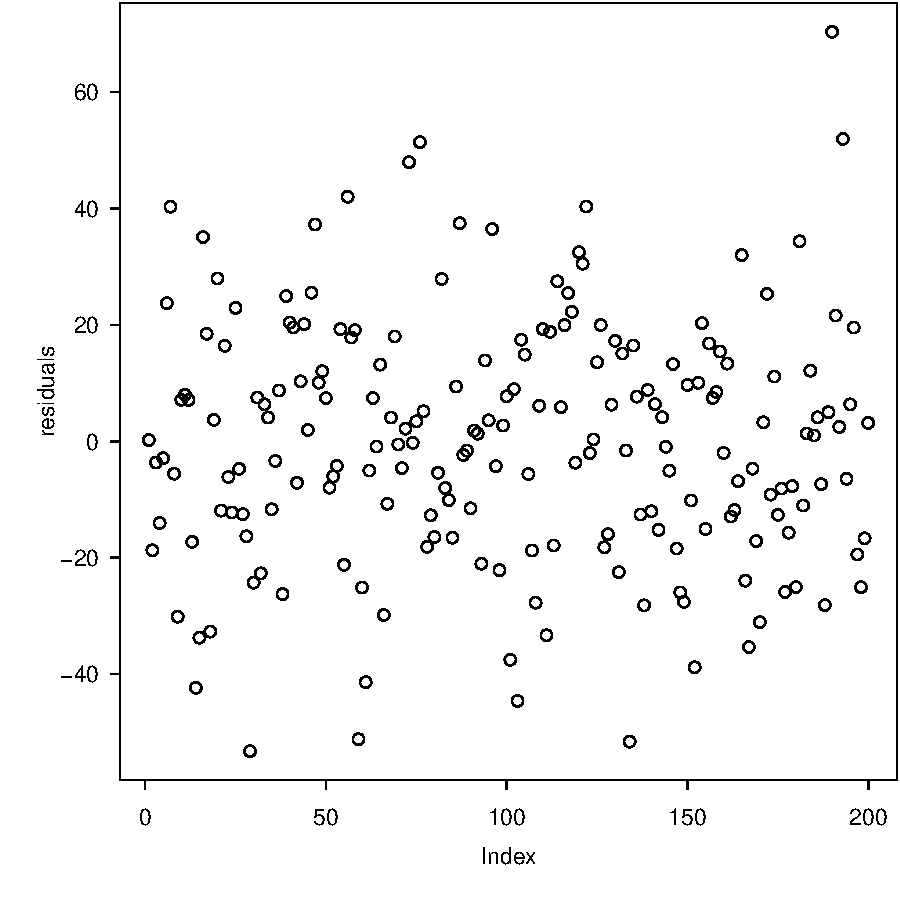
\includegraphics[width=.6\linewidth]{figure/r-codes-for-hw1-Rnwunnamed-chunk-2-1} 

}


\begin{kframe}\begin{alltt}
\hlcom{#The residuals plot shows that the mean is roughly 0, but it seems to have a polynomial pattern.}
\hlcom{#Since we do not have any information about the population distribution of the data, the use of GAM will be appropriate.}

\hlkwd{library}\hlstd{(gam)}
\end{alltt}


{\ttfamily\noindent\itshape\color{messagecolor}{\#\# Loading required package: splines}}

{\ttfamily\noindent\itshape\color{messagecolor}{\#\# Loading required package: foreach}}

{\ttfamily\noindent\itshape\color{messagecolor}{\#\# Loaded gam 1.20}}\begin{alltt}
\hlstd{gam1} \hlkwb{<-} \hlkwd{gam}\hlstd{(Y} \hlopt{~} \hlkwd{s}\hlstd{(X1,}\hlnum{2}\hlstd{)} \hlopt{+} \hlkwd{s}\hlstd{(X3,}\hlnum{2}\hlstd{),} \hlkwc{data} \hlstd{= q5)}
\hlkwd{par}\hlstd{(}\hlkwc{mfrow}\hlstd{=}\hlkwd{c}\hlstd{(}\hlnum{1}\hlstd{,}\hlnum{2}\hlstd{))}
\hlkwd{plot}\hlstd{(gam1)}
\end{alltt}
\end{kframe}

{\centering 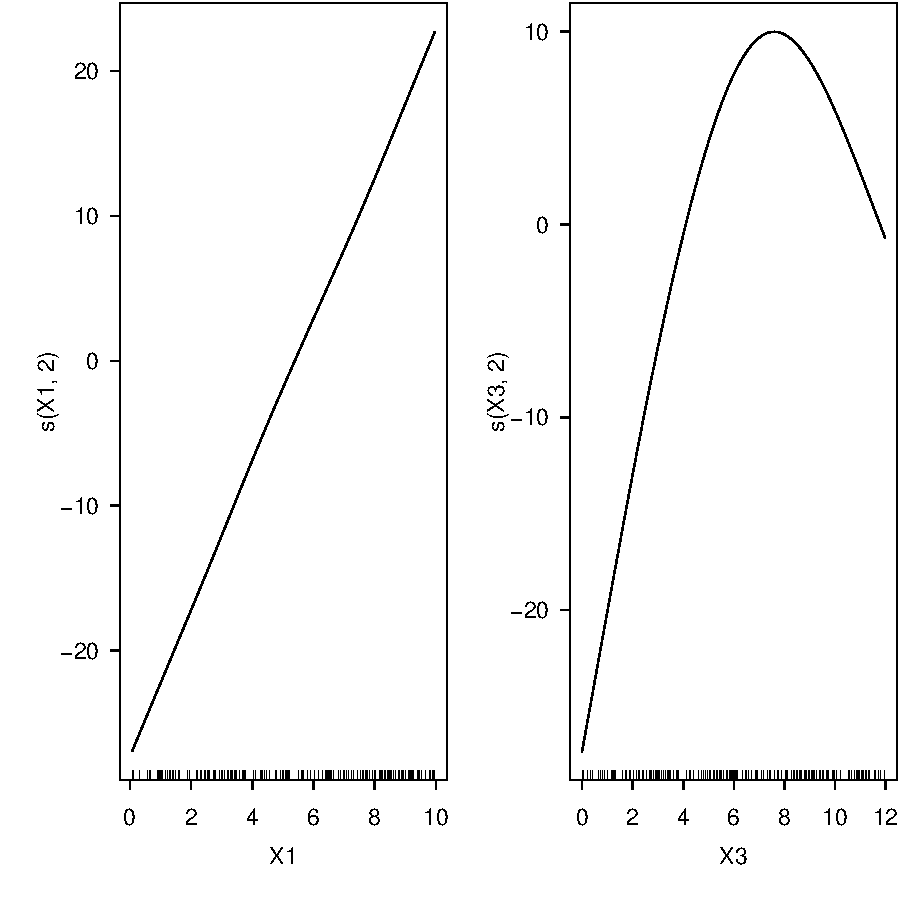
\includegraphics[width=.6\linewidth]{figure/r-codes-for-hw1-Rnwunnamed-chunk-2-2} 

}


\begin{kframe}\begin{alltt}
\hlkwd{par}\hlstd{(}\hlkwc{mfrow}\hlstd{=}\hlkwd{c}\hlstd{(}\hlnum{1}\hlstd{,}\hlnum{1}\hlstd{))}
\hlcom{# It is evident that the residuals of X1 variable are linear and those of the X3 variable are quadratic.}
\hlcom{# So we run a quadratic regression model. }
\hlkwd{library}\hlstd{(matrixcalc)}
\hlstd{f} \hlkwb{=} \hlkwa{function}\hlstd{(}\hlkwc{beta}\hlstd{,}\hlkwc{X}\hlstd{)}
\hlstd{\{}
  \hlstd{X1} \hlkwb{=} \hlstd{X[,}\hlnum{1}\hlstd{]; X3} \hlkwb{=} \hlstd{X[,}\hlnum{2}\hlstd{]}
  \hlstd{beta[}\hlnum{1}\hlstd{]} \hlopt{+} \hlstd{beta[}\hlnum{2}\hlstd{]}\hlopt{*}\hlstd{X1} \hlopt{+} \hlstd{beta[}\hlnum{3}\hlstd{]}\hlopt{*}\hlstd{X3} \hlopt{+} \hlstd{beta[}\hlnum{4}\hlstd{]}\hlopt{*}\hlstd{X3}\hlopt{^}\hlnum{2}
\hlstd{\}}
\hlstd{RSS} \hlkwb{=} \hlkwa{function}\hlstd{(}\hlkwc{beta}\hlstd{,}\hlkwc{Y}\hlstd{,}\hlkwc{X}\hlstd{)} \hlkwd{sum}\hlstd{((Y}\hlopt{-}\hlkwd{f}\hlstd{(beta,X))}\hlopt{^}\hlnum{2}\hlstd{)}
\hlstd{grv} \hlkwb{=} \hlkwa{function}\hlstd{(}\hlkwc{beta}\hlstd{,}\hlkwc{Y}\hlstd{,}\hlkwc{X}\hlstd{)}
\hlstd{\{}
  \hlstd{X1} \hlkwb{=} \hlstd{X[,}\hlnum{1}\hlstd{]; X3} \hlkwb{=} \hlstd{X[,}\hlnum{2}\hlstd{]}
  \hlstd{R} \hlkwb{=} \hlstd{Y} \hlopt{-} \hlkwd{f}\hlstd{(beta,X)}
  \hlkwd{c}\hlstd{(}\hlopt{-}\hlnum{2}\hlopt{*}\hlkwd{sum}\hlstd{(R),} \hlopt{-}\hlnum{2}\hlopt{*}\hlkwd{sum}\hlstd{(R}\hlopt{*}\hlstd{X1),} \hlopt{-}\hlnum{2}\hlopt{*}\hlkwd{sum}\hlstd{(R}\hlopt{*}\hlstd{X3),} \hlopt{-}\hlnum{2}\hlopt{*}\hlkwd{sum}\hlstd{(R}\hlopt{*}\hlstd{X3}\hlopt{^}\hlnum{2}\hlstd{))}
\hlstd{\}}

\hlstd{X} \hlkwb{=} \hlkwd{cbind}\hlstd{(q5}\hlopt{$}\hlstd{X1,q5}\hlopt{$}\hlstd{X3)}
\hlkwd{colnames}\hlstd{(X)} \hlkwb{=} \hlkwd{c}\hlstd{(}\hlstr{'X1'}\hlstd{,} \hlstr{'X3'}\hlstd{)}
\hlstd{Y} \hlkwb{=} \hlstd{q5}\hlopt{$}\hlstd{Y}
\hlstd{ml1} \hlkwb{=} \hlkwd{optim}\hlstd{(}\hlkwc{par} \hlstd{=} \hlkwd{rep}\hlstd{(}\hlnum{0.1}\hlstd{,}\hlnum{4}\hlstd{),} \hlkwc{fn} \hlstd{= RSS,} \hlkwc{gr}\hlstd{=grv,} \hlkwc{method}\hlstd{=}\hlstr{'BFGS'}\hlstd{,} \hlkwc{X}\hlstd{=X,} \hlkwc{Y}\hlstd{=Y)} \hlcom{#  par = initial Beta's, fn = optimize할 objective function, gr = gradient vector를 지정하는 함수}
\hlstd{ml1}
\end{alltt}
\begin{verbatim}
## $par
## [1] 31.6219679  4.8741981 13.8073463 -0.9626033
## 
## $value
## [1] 67981.31
## 
## $counts
## function gradient 
##       42        7 
## 
## $convergence
## [1] 0
## 
## $message
## NULL
\end{verbatim}
\begin{alltt}
\hlstd{beta.hat} \hlkwb{=} \hlstd{ml1}\hlopt{$}\hlstd{par}
\hlstd{beta.hat}
\end{alltt}
\begin{verbatim}
## [1] 31.6219679  4.8741981 13.8073463 -0.9626033
\end{verbatim}
\begin{alltt}
\hlstd{obj.mean} \hlkwb{=} \hlkwa{function}\hlstd{(}\hlkwc{beta}\hlstd{,}\hlkwc{Y}\hlstd{,}\hlkwc{X}\hlstd{,}\hlkwc{S}\hlstd{)} \hlkwd{t}\hlstd{(Y}\hlopt{-}\hlkwd{f}\hlstd{(beta,X))} \hlopt \hlkwd{solve}\hlstd{(S)} \hlopt \hlstd{(Y}\hlopt{-}\hlkwd{f}\hlstd{(beta,X))}
\hlstd{gr.mean} \hlkwb{=} \hlkwa{function}\hlstd{(}\hlkwc{beta}\hlstd{,}\hlkwc{Y}\hlstd{,}\hlkwc{X}\hlstd{,}\hlkwc{S}\hlstd{)}
\hlstd{\{}
  \hlstd{sigma2} \hlkwb{=} \hlkwd{diag}\hlstd{(S)}
  \hlstd{X1} \hlkwb{=} \hlstd{X[,}\hlnum{1}\hlstd{]; X3} \hlkwb{=} \hlstd{X[,}\hlnum{2}\hlstd{]}
  \hlstd{R} \hlkwb{=} \hlstd{Y} \hlopt{-} \hlkwd{f}\hlstd{(beta,X)}
  \hlkwd{c}\hlstd{(}\hlopt{-}\hlnum{2}\hlopt{*}\hlkwd{sum}\hlstd{(R),} \hlopt{-}\hlnum{2}\hlopt{*}\hlkwd{sum}\hlstd{(R}\hlopt{*}\hlstd{X1),} \hlopt{-}\hlnum{2}\hlopt{*}\hlkwd{sum}\hlstd{(R}\hlopt{*}\hlstd{X3),} \hlopt{-}\hlnum{2}\hlopt{*}\hlkwd{sum}\hlstd{(R}\hlopt{*}\hlstd{X3}\hlopt{^}\hlnum{2}\hlstd{))}
\hlstd{\}}

\hlstd{beta.new} \hlkwb{=} \hlstd{ml1}\hlopt{$}\hlstd{par}
\hlstd{W} \hlkwb{=} \hlkwd{diag}\hlstd{(}\hlkwd{rep}\hlstd{(}\hlnum{1}\hlstd{,}\hlkwd{length}\hlstd{(Y)))}
\hlstd{mdif} \hlkwb{=} \hlnum{100000}

\hlkwa{while}\hlstd{(mdif} \hlopt{>} \hlnum{0.000001}\hlstd{)}
\hlstd{\{}
  \hlstd{Yhat} \hlkwb{=} \hlkwd{f}\hlstd{(beta.new,X)}
  \hlstd{r} \hlkwb{=} \hlstd{Y} \hlopt{-} \hlstd{Yhat}
  \hlstd{Z} \hlkwb{=} \hlkwd{cbind}\hlstd{(}\hlnum{1}\hlstd{,Yhat)}
  \hlstd{gam.hat} \hlkwb{=} \hlkwd{solve}\hlstd{(}\hlkwd{t}\hlstd{(Z)} \hlopt \hlstd{W} \hlopt \hlstd{Z)} \hlopt \hlkwd{t}\hlstd{(Z)} \hlopt \hlstd{W} \hlopt \hlkwd{abs}\hlstd{(r)}
  \hlstd{sigma} \hlkwb{=} \hlstd{Z} \hlopt \hlstd{gam.hat}
  \hlstd{S} \hlkwb{=} \hlkwd{diag}\hlstd{(}\hlkwd{as.vector}\hlstd{(sigma}\hlopt{^}\hlnum{2}\hlstd{))}

  \hlkwa{if} \hlstd{(}\hlkwd{is.non.singular.matrix}\hlstd{(S)) W} \hlkwb{=} \hlkwd{solve}\hlstd{(S)}
  \hlkwa{else} \hlstd{W} \hlkwb{=} \hlkwd{solve}\hlstd{(S} \hlopt{+} \hlnum{0.000000001}\hlopt{*}\hlkwd{diag}\hlstd{(}\hlkwd{rep}\hlstd{(}\hlnum{1}\hlstd{,}\hlkwd{nrow}\hlstd{(S))))} \hlcom{#variance function구할 때의 weights}

  \hlstd{ml2} \hlkwb{=} \hlkwd{optim}\hlstd{(beta.new, obj.mean,} \hlkwc{gr}\hlstd{=gr.mean,}\hlkwc{method}\hlstd{=}\hlstr{'BFGS'}\hlstd{,} \hlkwc{Y}\hlstd{=Y,} \hlkwc{X}\hlstd{=X,} \hlkwc{S}\hlstd{=S)}
  \hlstd{beta.old} \hlkwb{=} \hlstd{beta.new}
  \hlstd{beta.new} \hlkwb{=} \hlstd{ml2}\hlopt{$}\hlstd{par}
  \hlstd{mdif} \hlkwb{=} \hlkwd{max}\hlstd{(}\hlkwd{abs}\hlstd{(beta.new} \hlopt{-} \hlstd{beta.old))}
\hlstd{\}}

\hlstd{beta.new}
\end{alltt}
\begin{verbatim}
## [1] 31.6219679  4.8741981 13.8073463 -0.9626033
\end{verbatim}
\begin{alltt}
\hlstd{Yhat} \hlkwb{=} \hlkwd{f}\hlstd{(beta.new,X)}
\hlstd{sigma} \hlkwb{=} \hlstd{Z} \hlopt \hlstd{gam.hat}
\hlstd{r} \hlkwb{=} \hlstd{(Y} \hlopt{-} \hlstd{Yhat)}\hlopt{/}\hlstd{sigma}

\hlcom{# Residual plot}
\hlkwd{plot}\hlstd{(Yhat,r)}
\end{alltt}
\end{kframe}

{\centering 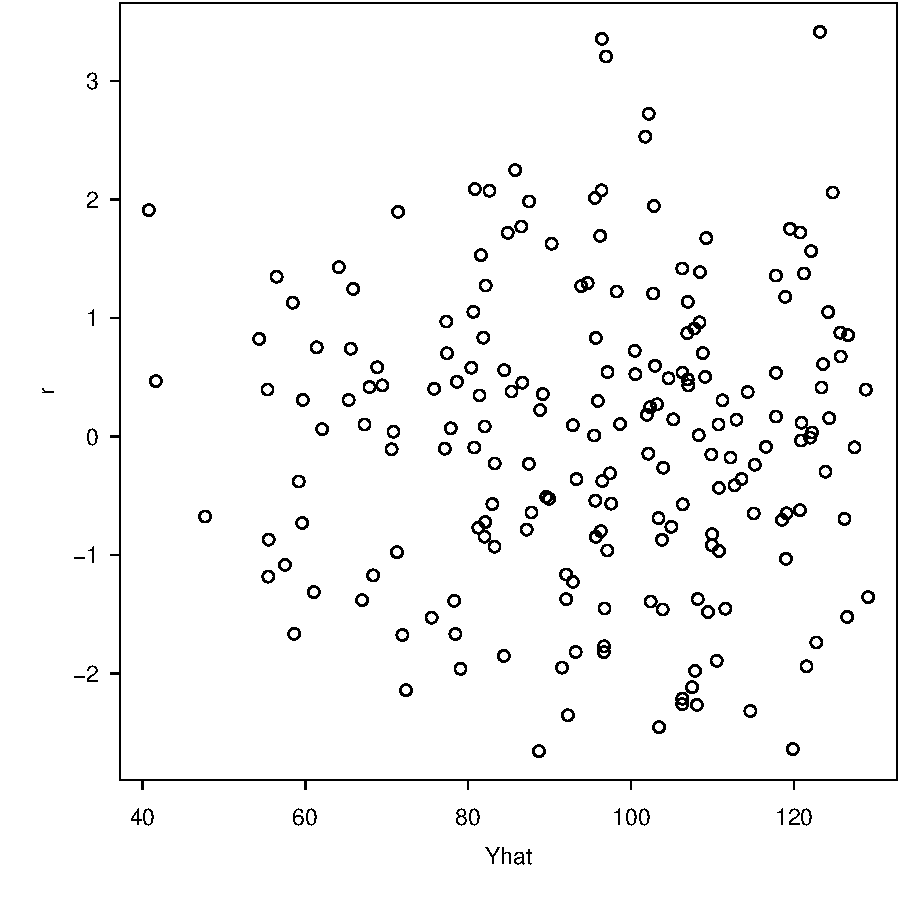
\includegraphics[width=.6\linewidth]{figure/r-codes-for-hw1-Rnwunnamed-chunk-2-3} 

}


\begin{kframe}\begin{alltt}
\hlcom{#The residuals seem to be centered around 0 and have a roughly uniform variance. }
\end{alltt}
\end{kframe}
\end{knitrout}

The R session information (including the OS info, R version and all
packages used):

\begin{knitrout}
\definecolor{shadecolor}{rgb}{0.969, 0.969, 0.969}\color{fgcolor}\begin{kframe}
\begin{alltt}
\hlkwd{sessionInfo}\hlstd{()}
\end{alltt}
\begin{verbatim}
## R version 4.1.1 (2021-08-10)
## Platform: aarch64-apple-darwin20 (64-bit)
## Running under: macOS Big Sur 11.6
## 
## Matrix products: default
## LAPACK: /Library/Frameworks/R.framework/Versions/4.1-arm64/Resources/lib/libRlapack.dylib
## 
## locale:
## [1] en_US.UTF-8/en_US.UTF-8/en_US.UTF-8/C/en_US.UTF-8/en_US.UTF-8
## 
## attached base packages:
## [1] splines   stats     graphics  grDevices utils     datasets  methods   base     
## 
## other attached packages:
## [1] matrixcalc_1.0-5 gam_1.20         foreach_1.5.1    spdep_1.1-11     sf_1.0-2        
## [6] spData_0.3.10    sp_1.4-5         tinytex_0.34    
## 
## loaded via a namespace (and not attached):
##  [1] Rcpp_1.0.7         compiler_4.1.1     highr_0.9          iterators_1.0.13  
##  [5] LearnBayes_2.15.1  class_7.3-19       tools_4.1.1        boot_1.3-28       
##  [9] digest_0.6.28      nlme_3.1-152       evaluate_0.14      lattice_0.20-44   
## [13] rlang_0.4.11       Matrix_1.3-4       DBI_1.1.1          yaml_2.2.1        
## [17] expm_0.999-6       xfun_0.26          fastmap_1.1.0      e1071_1.7-9       
## [21] coda_0.19-4        stringr_1.4.0      s2_1.0.6           raster_3.4-13     
## [25] knitr_1.36         gtools_3.9.2       classInt_0.4-3     grid_4.1.1        
## [29] rmarkdown_2.11     gdata_2.18.0       deldir_0.2-10      magrittr_2.0.1    
## [33] gmodels_2.18.1     codetools_0.2-18   htmltools_0.5.2    units_0.7-2       
## [37] MASS_7.3-54        KernSmooth_2.23-20 stringi_1.7.5      proxy_0.4-26      
## [41] wk_0.5.0
\end{verbatim}
\begin{alltt}
\hlkwd{Sys.time}\hlstd{()}
\end{alltt}
\begin{verbatim}
## [1] "2021-10-06 15:51:02 KST"
\end{verbatim}
\end{kframe}
\end{knitrout}


\end{document}
